\chapter{Experimental setup}
\label{chap:Experimentalsetup}


\section{Datasets}
\label{sec:datasets}

We use 5 datasets in our experiments, PowerDemand, SMTP, HTTP, SMTP+HTTP and ForestCover, those are widely used streaming datasets in the streaming data mining area \cite{encdecad}\cite{threaded}\cite{tan}. Statistical features are listed in  Table~\ref{tab:dataset}. PowerDemand is a small univariate time series that records the power demand over a period of one year. Weekdays’ demand is higher than weekends’ and daytime is higher than nights, demand of special days (e.g. festivals) are abnormal. The experimental data is an subsampling of original set. We demonstrate a synthetic example with visualization using this dataset while the trends and anomalous states are relative obviously. SMTP, HTTP, SMTP+HTTP are streaming anomaly data extracted from KDD Cup 99 dataset. According to Tan et al. \cite{tan}, HTTP contains sudden surges of anomalies and SMTP does not, but possibly exhibits some distribution changes within the stream. Because of the difficulty to point out where the distribution changes occur in the stream, the HTTP+SMPT dataset is derived by connecting SMTP and HTTP, so that a distribution change is occurred when the communication protocol is switched. The ForestCover dataset is from the UCI repository, which contains 6 kinds of forest cover types. Similar as Dong et al. \cite{threaded}, we defined the smallest class Cottonwood/Willow with 2747 instances as anomaly, and the rest 5 classes as normal class with distribution changes.

\begin{table}[ht] 
\caption{Datasets information} 
\centering      
\begin{tabular}{c c c c}  
\hline\hline        
Dataset & Size & Dimensionality & Anomaly proportion(\textperthousand) \\ [0.5ex] 
\hline 
PowerDemand & 35 040 & 1 &  21.92\\  
SMTP & 96 554 & 34 & 12.25  \\ 
HTTP & 623 091 & 34  & 6.49  \\ 
SMTP+HTTP & 719 645 & 34 & 7.26 \\ 
ForestCover & 581 012 & 7 & 3.53 \\ [1ex]  
\hline    
\end{tabular}
\label{tab:dataset}  
\end{table} 

We separate each dataset into initialization set and streaming set, both contain normal and abnormal data. Further, the initialization set is divided into 
\begin{itemize}
\item G(n\&a): for grid search
\item Tr(n): for model initial training
\item P(n\&a): for model parameter learning
\item Te(n\&a): for initial testing
\end{itemize}
where “n” represents normal data and “a” represents abnormal data. And the streaming set is published to Kafka to generate data stream (\Fref{fig:kafka}).

\begin{figure}[h]
\centering
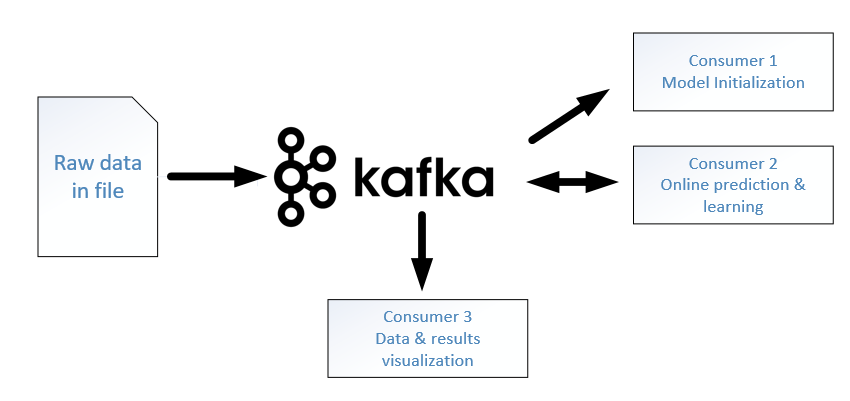
\includegraphics[width=10cm, height=5cm]{kafka}
\caption[Data stream Publisher-Consumer architecture]{Data stream Publisher-Consumer architecture}
\label{fig:kafka}
\end{figure}

For each dataset, we use half data for initialization and the other half for online prediction. The experimental results reported are averaged over 10 runs. For each run, the model is given with random initial weights. Each subset used for training and prediction are preprocessed with locally, in order to scale them into $[0,1]$ to fit the LSTM activation function.


\section{Parameter tuning}
\label{sec:parametertuning}

For each dataset, we carry out a grid search step to tuning the model hyperparameters that fit the data best. Here we try multiple combinations of window length and hidden size for each data set. The grid search set G contains 5\% -15\% anomalies, and same amount of normal data together with the anomalies make up the testing set in grid search. The rest normal data is used for training. Because of the uncertainty of the random neural network weight initialization, we do each experiment 10 times and take the average result to reduce the impact. To be noted that during every divisions, the consistency of streaming data is persisted, or in other words, no random sampling took place. A good model should make the reconstruction error as large as possible in order to make the classification easier. Given dataset D,  win is the input window, the average reconstruction error of D is given by \Fref{eq:are}. The target function of grid search is given by the ration of average reconstruction error of abnormal and normal test grid search set G (\Fref{eq:are}).

\begin{equation}\label{eq:are}
ARE(D) = \frac{1}{T}\sum_{t=1,win\in D}^{T}(input_{t,win}-output_{t,win})
\end{equation}

\begin{equation}\label{eq:ratio}
REratio=\frac{ARE(G_a)}{ARE(G_n)}
\end{equation}

\begin{figure}[h]
\centering
	\begin {subfigure}[t]{0.45\textwidth}
	\centering
	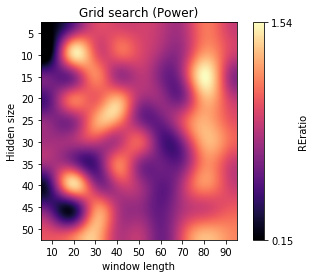
\includegraphics[height=6cm]{power_gridsearch}
	\caption{PowerDemand}
	\label{fig:power}
	\end{subfigure}
	~
	\begin {subfigure}[t]{0.45\textwidth}
	\centering
	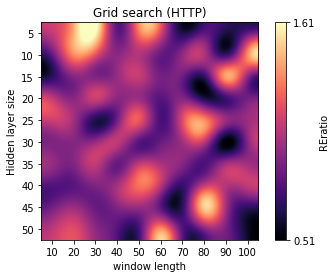
\includegraphics[height=6cm]{http_gridsearch}
	\caption{HTTP}
	\label{fig:http}
	\end{subfigure}
	~
	\begin {subfigure}[t]{0.45\textwidth}
	\centering
	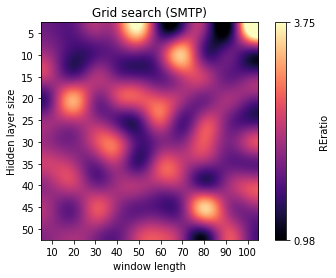
\includegraphics[ height=6cm]{smtp_gridsearch}
	\caption{SMTP}
	\label{fig:smtp}
	\end{subfigure}
	~
	\begin {subfigure}[t]{0.45\textwidth}
	\centering
	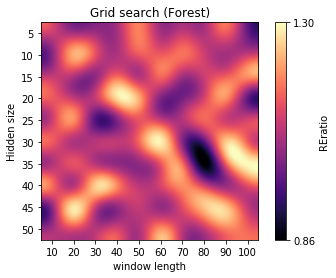
\includegraphics[height=6cm]{forest_gridsearch}
	\caption{Forest}
	\label{fig:forest}
	\end{subfigure}

	\caption[Grid search]{Grid search}
\label{fig:gridsearch}
\end{figure}

As a result of grid search, the hyperparameter for different datasets is listed in Table~\ref{tab:hyper}

\begin{table}[h] 
\caption{Hyperparameters} 
\centering      
\begin{tabular}{c c c c}  
\hline\hline        
Dataset & Window length & Hidden size & \#Grid Search instance \\ [0.5ex] 
\hline 
PowerDemand & 80 & 15 & 1 000 \\  
SMTP & 100 & 5 &  5 000 \\ 
SMTP+HTTP & 100 & 5 & 5 000 \\ 
HTTP & 30 & 5  &  10 000 \\ 
ForestCover & 100 & 35 & 10 000 \\ [1ex]  
\hline    
\end{tabular}
\label{tab:hyper}  
\end{table} 











